
\begin{tabular}{ccc}
\begin{tikzpicture}[
	dataBlob/.style={rectangle, anchor = center, node distance = 1cm},
	Layer/.style={rectangle, draw, anchor = center, fill=green!20, node distance = 1cm, minimum width=3.2cm},
	Activation/.style={rectangle, draw, anchor = center, fill=blue!20, node distance = 0.8cm},
	Misc/.style={rectangle, draw, anchor = center, fill=black!20, node distance = 1cm},
	bg/.style={rectangle, draw=red!40, line width = 2, anchor = north west,},
	myArrow/.style={->},
	myArrowR/.style={<-},
	label/.style={rectangle, anchor = center, node distance = 0.8cm},
	operator/.style={circle ,draw, anchor = center, minimum size = 0.2cm, inner sep = 0pt},
	Network/.style={rectangle, anchor = north west, minimum width = 2cm, fill = orange!40, draw, node distance = 1cm},
	]
%\node (topNet) [Network] at (-1,-1) {Encoder};
%\node (topInputGT) [dataBlob, xshift=-1cm] at([yshift=0.8cm]topNet.north) {$\original_\mathrm{top}$};
%\node (topInputRef) [dataBlob, xshift=1cm] at([yshift=0.8cm]topNet.north) {$\support_\mathrm{top}$};
%\draw[myArrow] (topInputGT.south) -- ([xshift=-1cm]topNet.north);
%\draw[myArrow] (topInputRef.south) -- ([xshift=1cm]topNet.north);

%\node (dummy1) [label] at (-0.5,0.2) {};
%\node (dummy1) [label] at (6.1,-6.5) {};

\draw [draw=black!60, line width=2] (-1.25,-0.45) rectangle (4.1,-6.05);

\node (input) [dataBlob] at (2.5,0) {$\curV$};
\node (inputP) [dataBlob] at (0,0) {$\predV$};

\node (EncP) [Network, below of = inputP, yshift=-0.7cm] {$\encoderNet[3,\predChannels,\predChannels]$};

\node (Enc) [Network, below of = input, yshift=-0.7cm] {$\encoderNet[3\!+\!3,64,64]$};
\node (AE) [Misc, below of = Enc] {AE};

\node (AD) [Misc, below of = AE, yshift=-0.1cm] {AD};
\node (Dec) [Network, below of = AD] {$\decoderNet[64\!+\!\predChannels,64,3]$};
\node (output) [dataBlob, below of = Dec, yshift=-0.7cm] {$\recV$};

\node (l) [dataBlob, xshift=0.8cm, yshift=-0.3cm] at (EncP.south) {$\latentPredV\approx\predBNV$};

\draw [myArrow] (input) -- (Enc);
\draw [myArrow] (inputP) -- ++(0,-0.9) -| ([xshift=-0.5cm]Enc);
\draw [myArrow] (inputP) -- (EncP);
\draw [myArrow,] (Enc) -- (AE);
\draw [myArrow,dashed] (AE) -- (AD);
\draw [myArrow,] (AD) -- (Dec);
\draw [myArrow,] (EncP) -- ++(0,-2.6) -| ([xshift=-0.5cm]Dec);
\draw [myArrow] (Dec) -- (output);


\end{tikzpicture} 
&
\begin{tikzpicture}[
dataBlob/.style={rectangle, anchor = center, node distance = 1cm},
Layer/.style={rectangle, draw, anchor = center, fill=green!20, node distance = 1cm, minimum width=3.2cm},
Activation/.style={rectangle, draw, anchor = center, fill=blue!20, node distance = 0.8cm},
Misc/.style={rectangle, draw, anchor = center, fill=black!20, node distance = 1cm},
bg/.style={rectangle, draw=red!40, line width = 2, anchor = north west,},
myArrow/.style={->},
myArrowR/.style={<-},
label/.style={rectangle, anchor = center, node distance = 0.8cm},
operator/.style={circle ,draw, anchor = center, minimum size = 0.2cm, inner sep = 0pt},
Network/.style={rectangle, anchor = north west, minimum width = 2cm, fill = orange!40, draw, node distance = 1cm},
]
%\node (topNet) [Network] at (-1,-1) {Encoder};
%\node (topInputGT) [dataBlob, xshift=-1cm] at([yshift=0.8cm]topNet.north) {$\original_\mathrm{top}$};
%\node (topInputRef) [dataBlob, xshift=1cm] at([yshift=0.8cm]topNet.north) {$\support_\mathrm{top}$};
%\draw[myArrow] (topInputGT.south) -- ([xshift=-1cm]topNet.north);
%\draw[myArrow] (topInputRef.south) -- ([xshift=1cm]topNet.north);

%\node (dummy1) [label] at (-0.5,0.2) {};
%\node (dummy1) [label] at (6.1,-6.5) {};

\draw [draw=black!60, line width=2] (-1.45,-0.45) rectangle (4.1,-6.05); 

\node (input) [dataBlob] at (2.5,0) {$\curV$};
\node (inputP) [dataBlob] at (0,0) {$\predV$};

\node (diff) [operator, below of = input, yshift=0.1cm] {$+$};

\node (EncP) [Network, below of = inputP, yshift=-0.7cm] {$\encoderNet[3,\predChannels,\predChannels]$};

\node (Enc) [Network, below of = input, yshift=-0.7cm] {$\encoderNet[3\!+\!3,64,64]$};
\node (AE) [Misc, below of = Enc] {AE};

\node (AD) [Misc, below of = AE, yshift=-0.1cm] {AD};
\node (Dec) [Network, below of = AD] {$\decoderNet[64\!+\!\predChannels,64,3]$};

\node (sum) [operator, below of = Dec, yshift=0.1cm] {$+$}; 

\node (output) [dataBlob, below of = Dec, yshift=-0.7cm] {$\recV$};

\node (l) [dataBlob, xshift=0.8cm, yshift=-0.3cm] at (EncP.south) {$\latentPredV\approx\predBNV$};

\draw [myArrow] (input) -- (diff);
\draw [myArrow] (inputP) -- ++(0,-0.9) -| ([xshift=-2cm]Enc);
\draw [myArrow] (inputP) -- ++(0,-0.9) -- node [below, pos=0.95] {$-$} (diff);
\draw [myArrow] (inputP) -- ++(0,-0.9) -| ++(-1.25, -1) |- (sum);
\draw [myArrow] (diff) -- (Enc);
\draw [myArrow] (inputP) -- (EncP);
\draw [myArrow,] (Enc) -- (AE);
\draw [myArrow,dashed] (AE) -- (AD);
\draw [myArrow,] (AD) -- (Dec);
\draw [myArrow,] (EncP) -- ++(0,-2.6) -| ([xshift=-0.5cm]Dec);
\draw [myArrow] (Dec) -- (sum);
\draw [myArrow] (sum) -- (output);


\end{tikzpicture} 
&
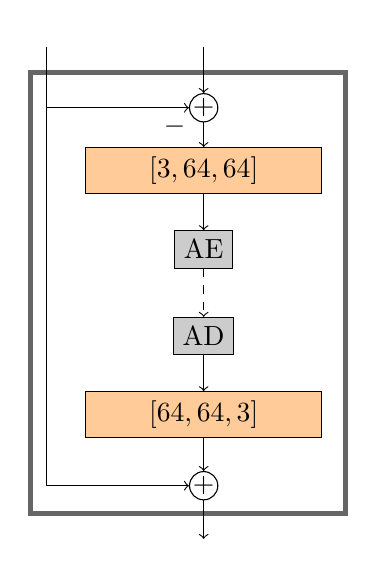
\begin{tikzpicture}[
dataBlob/.style={rectangle, anchor = center, node distance = 1cm},
Layer/.style={rectangle, draw, anchor = center, fill=green!20, node distance = 1cm, minimum width=3.2cm},
Activation/.style={rectangle, draw, anchor = center, fill=blue!20, node distance = 0.8cm},
Misc/.style={rectangle, draw, anchor = center, fill=black!20, node distance = 1cm},
bg/.style={rectangle, draw=red!40, line width = 2, anchor = north west,},
myArrow/.style={->},
myArrowR/.style={<-},
label/.style={rectangle, anchor = center, node distance = 0.8cm},
operator/.style={circle ,draw, anchor = center, minimum size = 0.2cm, inner sep = 0pt},
Network/.style={rectangle, anchor = north west, minimum width = 3cm, fill = orange!40, draw, node distance = 1cm},
]
%\node (topNet) [Network] at (-1,-1) {Encoder};
%\node (topInputGT) [dataBlob, xshift=-1cm] at([yshift=0.8cm]topNet.north) {$\original_\mathrm{top}$};
%\node (topInputRef) [dataBlob, xshift=1cm] at([yshift=0.8cm]topNet.north) {$\support_\mathrm{top}$};
%\draw[myArrow] (topInputGT.south) -- ([xshift=-1cm]topNet.north);
%\draw[myArrow] (topInputRef.south) -- ([xshift=1cm]topNet.north);

%\node (dummy1) [label] at (-0.5,0.2) {};
%\node (dummy1) [label] at (6.1,-6.5) {};

\draw [draw=black!60, line width=2] (-2.2,-0.45) rectangle (1.8,-6.05);

\node (input) [dataBlob] at (0,0) {$\curV$};
\node (inputP) [dataBlob] at (-2,0) {$\predV$};

\node (diff) [operator, below of = input, yshift=0.1cm] {$+$}; 

\node (Enc) [Network, below of = input, yshift=-0.7cm] {$\encoderNet[3,64,64]$};
\node (AE) [Misc, below of = Enc] {AE};
\node (AD) [Misc, below of = AE, yshift=-0.1cm] {AD};
\node (Dec) [Network, below of = AD] {$\decoderNet[64,64,3]$};
\node (output) [dataBlob, below of = Dec, yshift=-0.7cm] {$\recV$};
\node (sum) [operator, below of = Dec, yshift=0.1cm] {$+$}; 

\draw [myArrow] (input) -- (diff);
\draw [myArrow] (inputP) |- node [below, pos=0.95] {$-$} (diff);
\draw [myArrow] (diff) -- (Enc);
\draw [myArrow,] (Enc) -- (AE);
\draw [myArrow,dashed] (AE) -- (AD);
\draw [myArrow,] (AD) -- (Dec);
\draw [myArrow] (Dec) -- (sum);
\draw [myArrow] (inputP) |- (sum);
\draw [myArrow] (sum) -- (output);

\end{tikzpicture}		
\\
(a) Conditional Coder~\cite{LadunePH2020_ModeNetModeSelection} & (b) Conditional Residual Coder & (c) Equivalent Residual Coder
\end{tabular}